% !TEX root = ./Vortrag.tex
\begin{frame}[label=title]{}
\titlepage
\begin{center} Betreuer: Benjamin Reh \& Thomas Kloepfer
\end{center}
\end{frame}
\begin{frame}[label=title]{}
\tableofcontents
\end{frame}

\section{Projektziel}
\begin{frame}{Projektziel}
\begin{exampleblock}{Zielvorgaben}
\begin{itemize}
\item Konstruktion eines autonomen Fahrzeugs
\begin{itemize}
\item Fahrt nach GPS-Daten
\item Ausweichen kleinerer Hindernises
\end{itemize}
\end{itemize}
\end{exampleblock}
\\[0.5cm]
\begin{exampleblock}{Umsetzung}
\begin{itemize}
\item Umbau eines Modellautos
\item Steuerung durch einen Raspberry Pi
\item Erkennen der Hindernisse durch Ultraschallsensoren
\item GPS Modul mit Kompass
\item Programmierung in Python
\end{itemize}
\end{exampleblock}
\end{frame}

% Local background must be enclosed by curly braces for grouping.
%{
%\usebackgroundtemplate{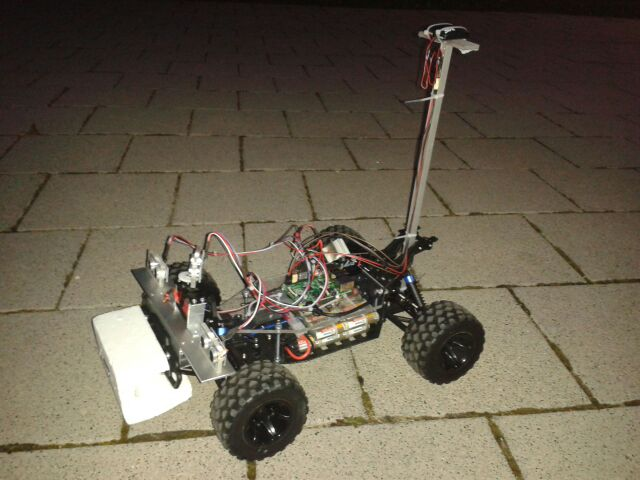
\includegraphics[height=\textheight]{Plots/new_design_IV.JPG}}%
\begin{frame}{Komponenten}
\vspace*{-.5cm}
\begin{figure}
\center
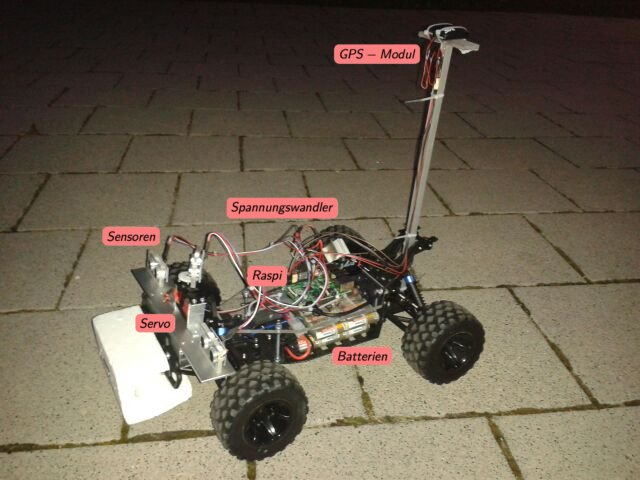
\includegraphics[height=\textheight]{Plots/new_design_IV_new.JPG}
\end{figure}
%\begin{tikzpicture}
%	\node[inner sep=0pt,remember picture,overlay] at (9,-2.3){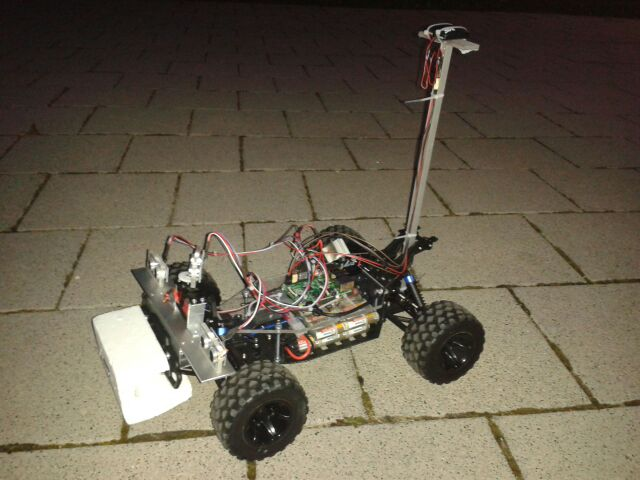
\includegraphics[height=.9\textheight]{Plots/new_design_IV.JPG}};
%	\node (Raspi) at (7.5,-2.5) [rounded corners=4pt, fill=red!50] {$Raspi$};
%	\node (Servo) at (4,-3) [rounded corners=4pt, fill=red!50] {$Servo$};
%	\node (Sensoren) at (4,-4) [rounded corners=4pt, fill=red!50] {$Sensoren$};
%	\node (GPS-Modul) at (9,1) [rounded corners=4pt, fill=red!50] {$GPS-Modul$};
%	\node (Batterien) at (7.5,-4.2) [rounded corners=4pt, fill=red!50] {$Batterien$};
%	\node (Spannungswandler) at (8,-2) [rounded corners=4pt, fill=red!50] {$Spannungswandler$};
%\end{tikzpicture}
\end{frame}%}

\section{Aufbau des Autos}

\begin{frame}{Aufbau des Autos}
\begin{itemize}
\item Bausatz des Modellautos
\item Plexiglasplatte für Raspi, Spannungswandler, usw.
\item Ansteuerung des Fahrtreglers und der Servos
\item Auslesen und Ansteuern von GPS und Ultraschallsensoren
\item Erarbeitung eines Navigationskonzepts
\item Entwicklung und Optimierung des Ausweichalgorithmus
\item Implementierung von GPS und Kompass ins Fahrtkonzept
\item Optisches Tuning
\item Fehlerbehebung/Verbesserungen
\end{itemize}
\end{frame}

\section{Features}
\begin{frame}{Features}
\begin{itemize}
\item Kommunikation via WLAN
\item Verschiedenen Output-Level zum Debuggen
\item Erstellen von Logfiles (GPS + Output) für Plots in Google Maps
\item GPS und Sensoren in Background-Threads 
\item Verschiedene Modi für den schwenkbaren Sensor
\item Findet günstigsten Weg bei vielen Hindernissen
\item Getrennte Spannungsversorgung
\end{itemize}
\end{frame}

\section{Programmstruktur}
\begin{frame}{Programmstruktur}
\vspace*{-.5cm}
\begin{figure}
\center
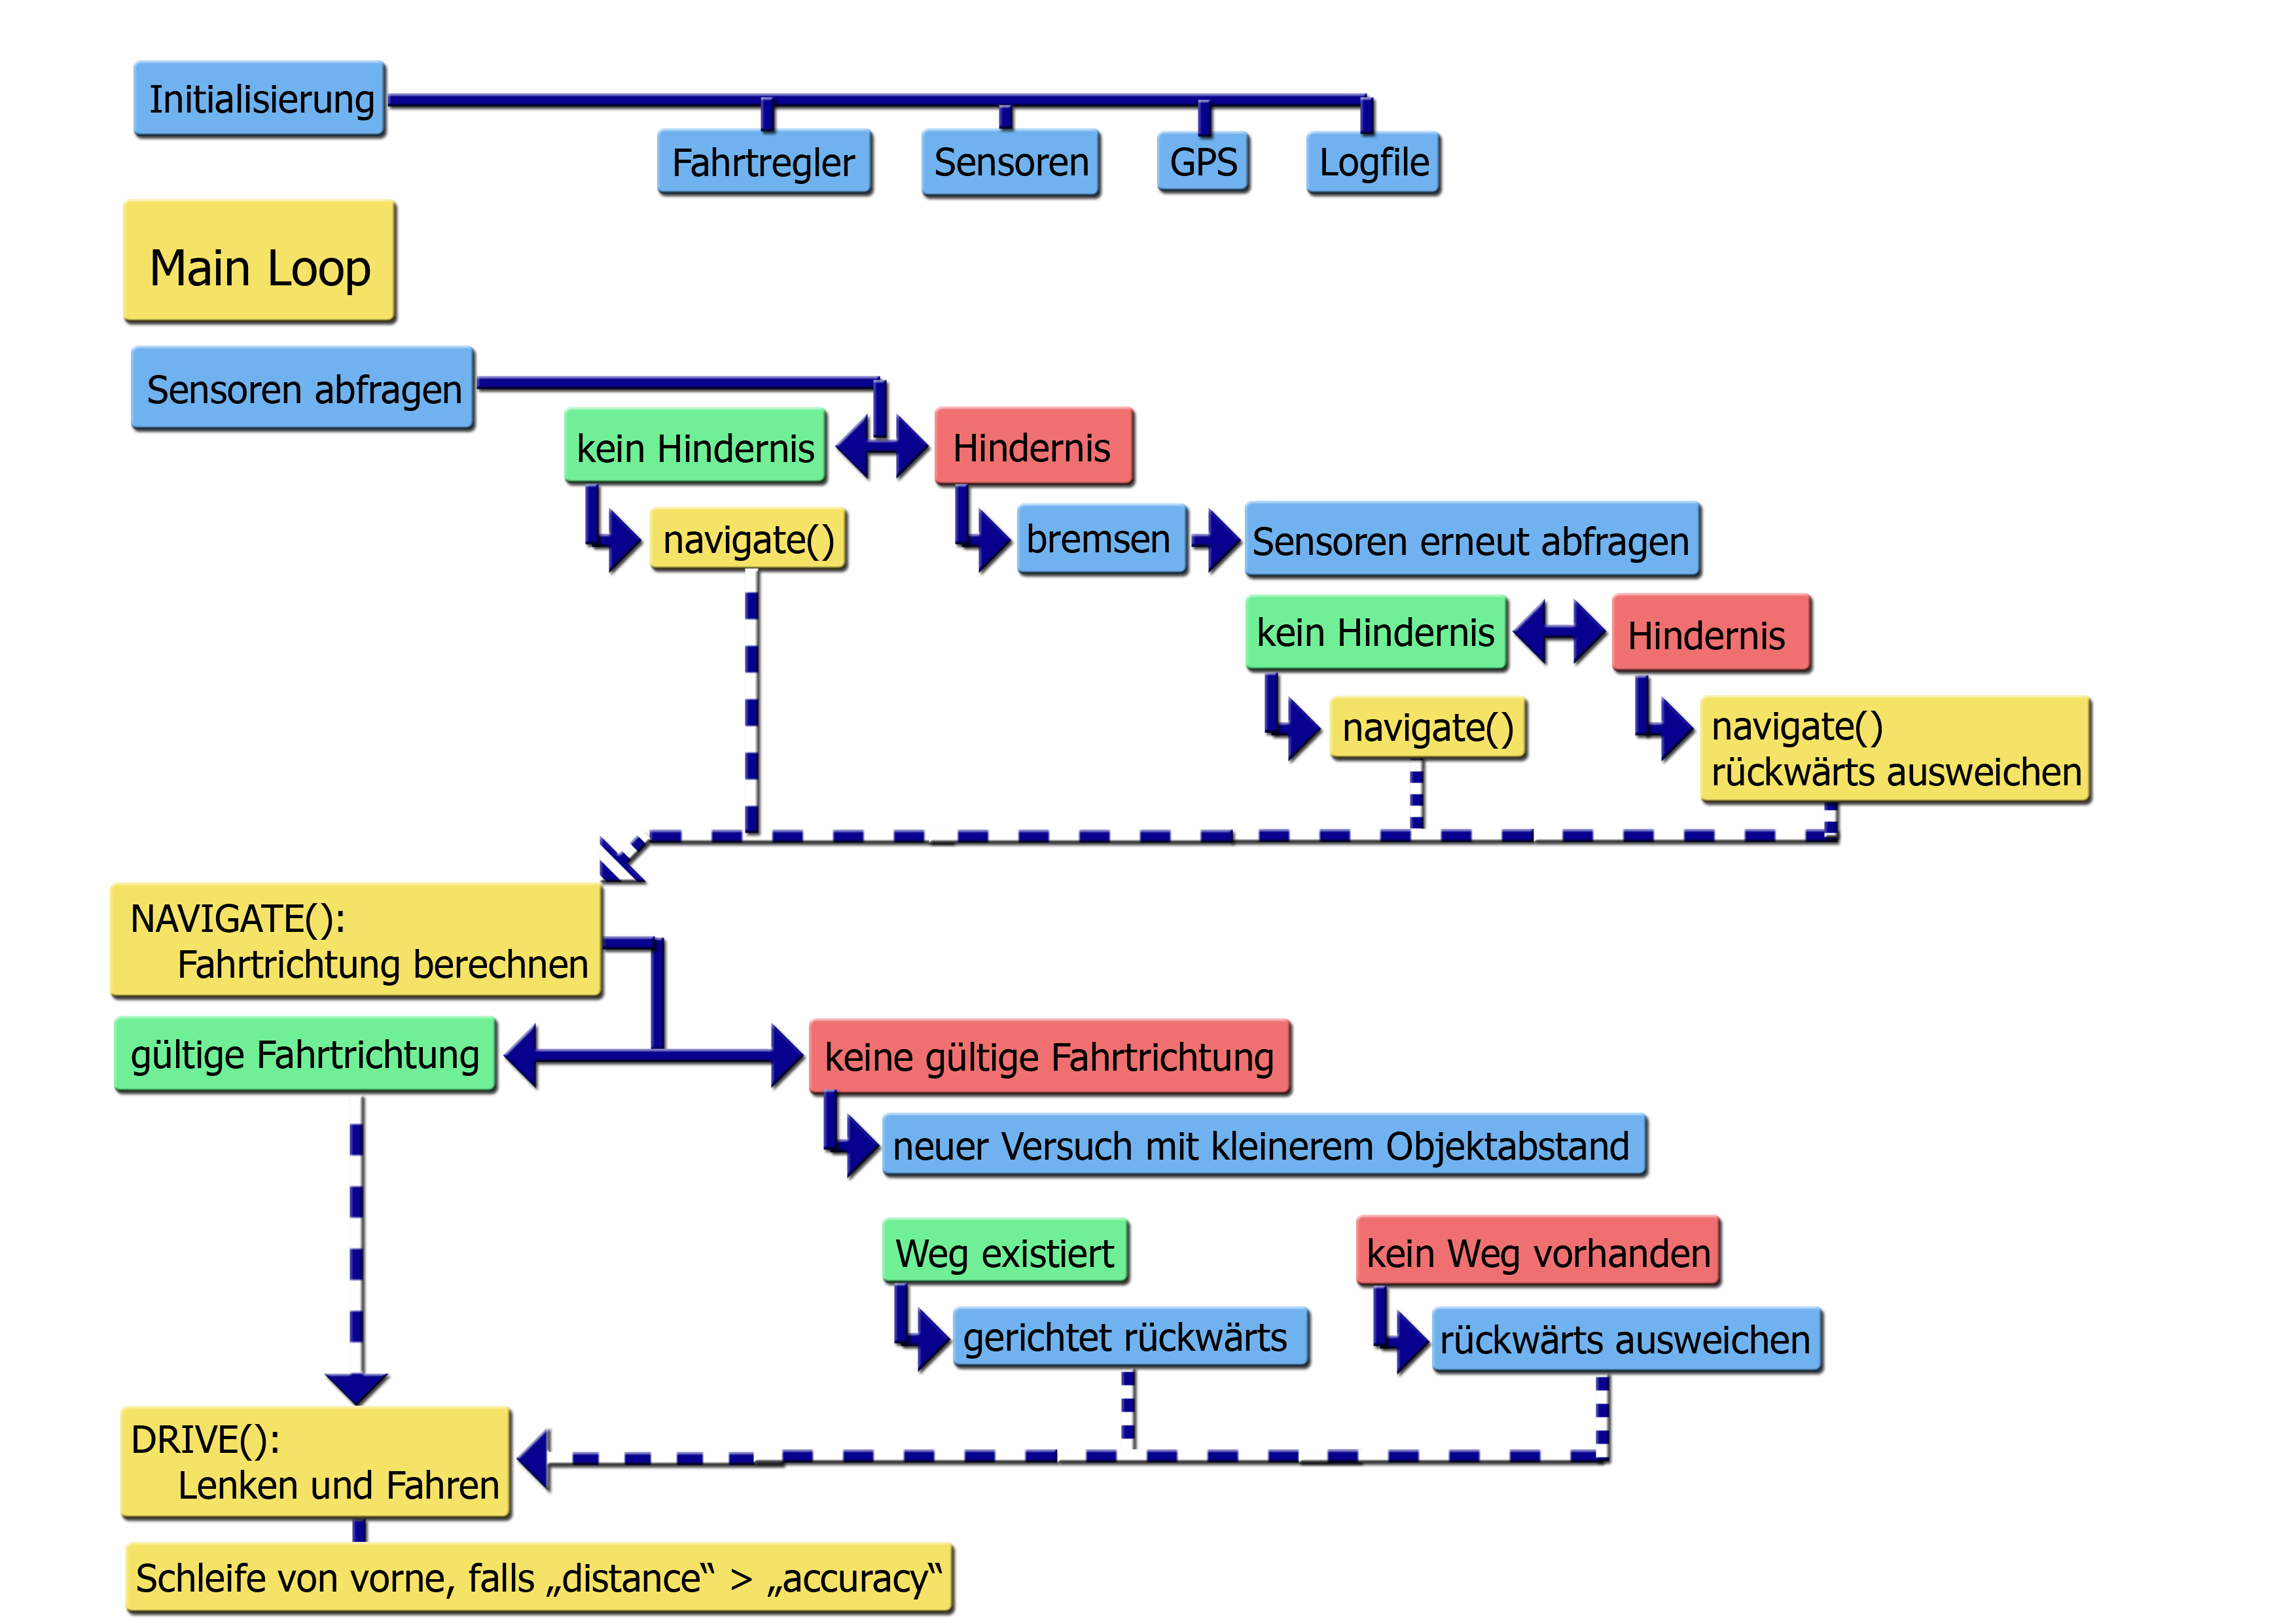
\includegraphics[height=.9\textheight]{Plots/Flowchart}
\end{figure}
\end{frame}


\begin{frame}{Navigation}
\begin{columns}
\column{0.49\paperwidth}
\vspace{-0.5cm}
\begin{figure}
\center
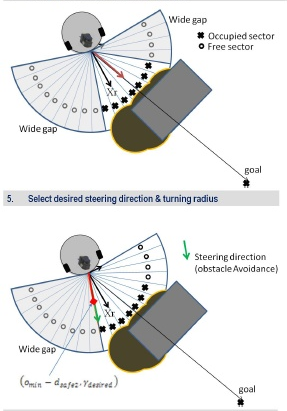
\includegraphics[height=.85\textheight]{Plots/navigation1}
\end{figure}
\column{0.49\paperwidth}
\begin{itemize}
\item Sensoren abfragen
\item Richtung zum Ziel vom GPS/Kompass
\\[1cm]
\item freie Segmente finden
\item Einteilung in große, mittlere und kleine Lücken
\end{itemize}
\end{columns}
\end{frame}

\begin{frame}{Navigation}
\begin{columns}
\column{0.49\paperwidth}
\vspace{-0.5cm}
\begin{figure}
\center
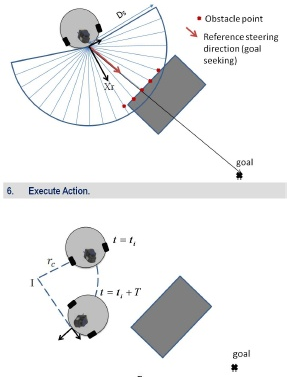
\includegraphics[height=.85\textheight]{Plots/navigation2}
\end{figure}
\column{0.49\paperwidth}
\begin{itemize}
\item Lenkrichtung anhand einer Kostenfunktion errechnen
\item $Cost = c_1 (r_{ref} - r_{gap}) + c_2 d_{gap}$
\\[1cm]
\item in errechnete Richtung ausweichen
\end{itemize}
\end{columns}
\end{frame}

\begin{frame}{Sensor-Thread}
\begin{itemize}
\item Abfragereihenfolge: links, oben, rechts, oben, links, ...
\item Bei Abfrage oben, drehe den Servo weiter nach rechts
\item Am rechten Rand, springe nach links \\[0.5cm]
\item Speichere aktuelle Sensordaten in Array
\item Ignoriere Werte kleiner als 7cm
\item Fünf Versuche für korrekte Messung
\end{itemize}
\end{frame}


\begin{frame}[containsverbatim]{Sensor-Thread}
%\vspace{-1cm}
\begin{columns}
\column{0.49\paperwidth}
\begin{lstlisting}[tabsize=2, basicstyle=\ttfamily\scriptsize]
def get_distance(i):
	GPIO.setmode(GPIO.BCM)

	TRIG = [15, 8, 7]  
	ECHO = [14, 9, 11] 

	GPIO.setup(TRIG[i], GPIO.OUT)
	GPIO.setup(ECHO[i], GPIO.IN)

	GPIO.output(TRIG[i], False)

	time.sleep(.04)

	GPIO.output(TRIG[i], True)
	time.sleep(0.00001)
	GPIO.output(TRIG[i], False)
\end{lstlisting}	
\column{0.49\paperwidth}
\begin{lstlisting}[tabsize=2, basicstyle=\ttfamily\scriptsize]
	while (GPIO.input(ECHO[i])!=1):
		start_time = time.time()
	
	while (GPIO.input(ECHO[i])==1):
		dt = time.time() - start_time
		if(dt>0.05):
			return 10000000.0

	dist = dt*17000.0
	time.sleep(.04)
	return dist
\end{lstlisting}
\end{columns}
\end{frame}

\section{Probleme}

\begin{frame}{Probleme}
\begin{itemize}
\item Spannungsversorgung
\item defekte Bauteile und Lieferschwierigkeiten
\item Ultraschallsensoren
\item GPS-Genauigkeit und Kompass
\item Testfahrten
\end{itemize}
\end{frame}

\section{Ausblick}

\begin{frame}{Ausblick}
\begin{itemize}
\item feinere Motor- und Sensoransteuerung, schnellere Sensorabfrage
\item Verbesserung des GPS
\item bessere Sensoren
\item Verfeinerung des Navigationsalgorithmus
\item Benutzeroberfläche (z.B. Webpage zur Steuerung)
\item interne Karte bzw. Einbindung von OpenStreetMaps
\end{itemize}
\end{frame}

\begin{frame}
\begin{center}
\textcolor{darkred}{
Vielen Dank für Ihre Aufmerksamkeit
\\[1cm]
Es folgt GPS auf Rädern B}
\end{center}
\end{frame}
